\documentclass[14pt,a4paper]{extreport}

\usepackage{style/style}
\usepackage{physics}
\usepackage{fancyhdr}
\usepackage{pdfpages}

\fancypagestyle{plain}{%
\fancyhf{} % clear all header and footer fields
\fancyfoot[C]{\small\thepage}}
\renewcommand{\headrulewidth}{0pt}
\renewcommand{\footrulewidth}{0pt}
\pagestyle{plain}

\makeatletter
  \def\my@tag@font{\small}
  \def\maketag@@@#1{\hbox{\m@th\normalfont\my@tag@font#1}}
  \let\amsmath@eqref\eqref
  \renewcommand\eqref[1]{{\let\my@tag@font\relax\amsmath@eqref{#1}}}
\makeatother

\usepackage{titletoc}
\titlecontents{chapter}[0em]{\bfseries}{\thecontentslabel.\hspace{1em}}{}{\titlerule*[1pc]{.}\contentspage}
\titlecontents{section}[1.25em]{}{\thecontentslabel.\hspace{1em}}{}{\titlerule*[1pc]{.}\contentspage}
\titlecontents{subsection}[2.5em]{}{\thecontentslabel.\hspace{1em}}{}{\titlerule*[1pc]{.}\contentspage}

\begin{document}

%\includepdf[pages=-]{Title.pdf}
%\includepdf[pages=-]{Task_list.pdf}

% Отключение нумерации страниц
\pagenumbering{gobble}

%\chapter*{Аннотация}

Отчёт 91 с., 4 ч., 24 рис., 26 табл., 13 источников, 1 прил.

ЧИСЛЕННОЕ МОДЕЛИРОВАНИЕ ЭЛЕКТРОМАГНИТНОГО \\ ПОЛЯ, МЕТОД КОНЕЧНЫХ ЭЛЕМЕНТОВ, МНОГОЭТАПНАЯ СХЕМА РАЗДЕЛЕНИЯ ПОЛЕЙ

Цель работы: разработка программы для численного моделирования нестационарного электромагнитного поля в трёхмерной среде, создаваемого индукционным источником тока, при помощи многоэтапной схемы разделения полей.

В процессе работы был разработан и протестирован  программный модуль численного моделирования электромагнитного поля с помощью многоэтапной схемы разделения полей.

С помощью программы проводилось исследование поведения поля в приповерхностных слоях земной коры с различными значениями удельной электропроводности горизонтально-слоистой среды и аномальных объектов. 

\newpage

\tableofcontents
\newpage

% Включение нумерации страниц
\pagenumbering{arabic}
\setcounter{page}{3}
%\chapter*{Введение}

\addcontentsline{toc}{chapter}{Введение}

Разработка программного обеспечения для моделирования трехмерного электромагнитного поля представляет собой сложную и актуальную задачу, особенно в контексте современных требований к точности и эффективности расчетов. Одним из перспективных подходов к решению таких задач является использование векторного метода конечных элементов (МКЭ), который обеспечивает высокую точность моделирования. 

В данной работе рассматривается разработка программы для моделирования электромагнитного поля на шестигранных элементах, что особенно важно для задач, связанных с анализом поведения электромагнитного поля в электроразведке. Применение шестигранников в качестве базовых элементов сетки позволяет более гибко аппроксимировать сложные трехмерные структуры, что делает данный подход особенно востребованным для решения практических задач.
%\chapter{Постановка задачи}

\section{Аппарат математического моделирования}

Математическая модель, описывающая поведение электромагнитного поля в пространстве, известна в наши дни, как система уравнений Максвелла. Она позволяет описывать взаимосвязь сразу нескольких физических величин: напряжённости электрического $\overrightarrow{\textbf{E}}$ и магнитного $\overrightarrow{\textbf{H}}$ полей, а также индукцию магнитного поля $\overrightarrow{\textbf{B}}$. Большинство вычислительных задач электромагнетизма базируются на дифференциальной форме системы уравнений Максвелла:

\begin{equation} \label{eq_1_1}
	\text{rot} \overrightarrow{\textbf{H}} = \overrightarrow{\textbf{J}^{\text{ст}}} + \sigma \overrightarrow{\textbf{E}} + \frac{\partial \left(\varepsilon \overrightarrow{\textbf{E}} \right)}{\partial t},
\end{equation}

\begin{equation} \label{eq_1_2}
	\text{rot} \overrightarrow{\textbf{E}} = - \frac{\partial \overrightarrow{\textbf{B}}}{\partial t},
\end{equation}

\begin{equation} \label{eq_1_3}
	\text{div} \overrightarrow{\textbf{B}} = 0,
\end{equation}

\begin{equation} \label{eq_1_4}
	\text{div} \varepsilon \overrightarrow{\textbf{E}} = \rho,
\end{equation}
где $\overrightarrow{\textbf{J}^{\text{ст}}}$ -- вектор плотностей сторонних токов, $\sigma$ -- удельная электрическая проводимость среды, $\varepsilon$ -- диэлектрическая проницаемость среды, а $\rho$ -- объёмная плотность стороннего электрического заряда.

Основное преимущество использования системы уравнений (\ref{eq_1_1}) -- (\ref{eq_1_4}) в дифференциальной форме, заключается в возможности учитывать нелинейность, анизотропию и другие нетривиальные аспекты среды \cite{3}. 

Пусть электромагнитное поле возбуждается индукционным источником. В таком случае, при отсутствии аномальных объектов, будем решать задачу в цилиндрических координатах. Источник поля в таком случае описывается точкой, расположенной на некотором расстоянии, достаточно далёком от границы расчётной области. Тогда при условии однородности среды по магнитной проницаемости и отстутствия токов смещения электромагнитное поле полностью описывается одной компонентой $A_{\varphi} = A_{\varphi}(r, z, t)$ вектор-потенциала $\overrightarrow{\textbf{A}}$. Функция $A_{\varphi}(r, z, t)$ может быть найдена из решения двумерного уравнения (\ref{eq_1_5}):

\begin{equation} \label{eq_1_5}
	-\frac{1}{\mu_0} \Delta A_{\varphi} + \frac{A_{\varphi}}{\mu_0 r^2} + \sigma \frac{\partial A_{\varphi}}{\partial t} = J_{\varphi},
\end{equation}
где $\mu_0 = 4 \cdot \pi \cdot 10^{-7} = 1.25663753 \cdot 10^{-6}$ Гн/м -- магнитная постоянная, $J_{\varphi}$ - источник стороннего тока, описываемый дельта-функцией, равной 1 в одной из подобласти, описывающей источник поля, и 0 во всех остальных \cite{4}. Удельную электропроводность $\sigma$ представим в виде кусочно-постоянной функции, описывающей физические характеристики горизонтально-слоистой среды. Потребуем, чтобы на всех границах было главное краевое условие $\left.A_{\varphi}(r, z, t)\right|_s = 0$. Тогда решение задачи (\ref{eq_1_5}) с главными однородными условиями на границах будем называть первичным или нормальным полем.

Решением задачи на оценку влияния аномальных объектов в горизонтально-слоистой среде будем называть вторичным (добавочным) полем. Также, как и в (\ref{eq_1_5}) потребуем на всех границах главное однородное краевое условие $\overrightarrow{\textbf{A}} \times \overrightarrow{\textbf{n}} |_s = 0$. Тогда, нестационарный процесс, возникающий после выключения источника тока в круглой обмотке, описывается следствием из уравнения (\ref{eq_1_1}) \cite{5}:

\begin{equation} \label{eq_1_6}
	\text{rot} \left( \frac{1}{\mu_o} \text{rot} \overrightarrow{\textbf{A}}^{+} \right) + \sigma \frac{\partial \overrightarrow{\textbf{A}}^{+}}{\partial t} = (\sigma - \sigma_n) \overrightarrow{\textbf{E}}^n,
\end{equation}
где $\sigma_n$ -- значение удельной электрической проводимости среды на нормальном слое, $\overrightarrow{\textbf{E}}^n$ -- напряжённость первичного электрического поля, $\overrightarrow{\textbf{A}}^{+}$ -- значение вектор-потенциала на добавочном поле.

\section{Описание расчётной области}

Пусть у нас имеется расчётная область, геометрически представленная в виде параллелепипеда: $\Omega \in [-55000, 55000]_x \times [-55000, 55000]_y \times [-25000, 25000]_z$. Внутри неё имеются слои воздуха, и некоторых пород верхних слоёв земной коры. Тогда половина продольного диагонального среза горизонтально-слоистой среды изображена на рисунке \ref{fig:example}. Будем её использовать в качестве расчётной области для двумерной задачи. В среде, обозначенной коричневым цветом задано значение $\sigma_1 = 0.01$ См/м, в бледной $\sigma_2 = 0.005$ См/м и в зелёной $\sigma_3 = 0.001$ См/м. Поскольку воздух является диэлектриком, значение удельной электропроводности для него $\sigma_{\text{возд.}} = 0$ См/м.

\begin{figure}
	\centering
	\vspace*{0.7cm}
	\includegraphics[width=1.0\linewidth]{images/"Figure_example".png}
	\caption{Срез горизонтально-слоистой среды}
	\label{fig:example}
\end{figure}
\chapter{Теоретическая часть}

\section{Векторные дифференциальные уравнения второго порядка с разрывными решениями}

Математическая модель, служащая для описания электромагнитного поля в средах с изменяющимся коэффициентом магнитной проницаемости и в ситуациях, когда нельзя пренебрегать влиянием токов смещения, выглядит следующим образом (\ref{eq_1_1}):

\begin{equation} \label{eq_1_1}
	\text{rot} \left( \frac{1}{\mu} \text{rot} \overrightarrow{\textbf{A}} \right) + \sigma \frac{\partial \overrightarrow{\textbf{A}}}{\partial t} + \epsilon \frac{\partial^2 \overrightarrow{\textbf{A}}}{\partial t^2} = \overrightarrow{\textbf{J}}^{\textbf{ст}}.
\end{equation}

Математическая модель электромагнитного поля на основе уравнения (\ref{eq_1_1}) позволяет решать самые сложные задачи электромагнетизма. Она корректно описывает электромагнитные поля в ситуациях, когда среда содержит любые неоднородности с измененными электрическими и магнитными свойствами.

При решении задач с использованием схемы разделения полей, для описания осесимметричной горизонтально-слоистой среды используется следующее уравнение (\ref{eq_1_2}):

\begin{equation} \label{eq_1_2}
	-\frac{1}{\mu_0} \Delta A_{\varphi} + \frac{A_{\varphi}}{\mu_0 r^2} + \sigma \frac{\partial A_{\varphi}}{\partial t} = J_{\varphi}.
\end{equation}

В свою очередь, учёт от объектов, имеющих неоднородные значения удельной электропроводности, осуществляется за счёт математической модели, описываемой уравнением (\ref{eq_1_3})

\begin{equation} \label{eq_1_3}
	\text{rot} \left( \frac{1}{\mu_0} \text{rot} \overrightarrow{\textbf{A}}^+ \right) + \sigma \frac{\partial \overrightarrow{\textbf{A}}^+}{\partial t} = \left( \sigma - \sigma_{\text{n}} \right) \overrightarrow{\textbf{E}}_{\text{n}}.
\end{equation}

Для тестирования на правильность решения дифференциального уравнения (\ref{eq_1_3}) будем использовать уравнение (\ref{eq_1_4}), правая часть которого представляется в виде вектор-функции $\overrightarrow{\textbf{F}}$, а также будет иметь место быть слагаемое $\gamma \overrightarrow{\textbf{A}}$ в левой части уравнения:

\begin{equation} \label{eq_1_4}
	\text{rot} \left( \frac{1}{\mu_0} \text{rot} \overrightarrow{\textbf{A}} \right) + \gamma \overrightarrow{\textbf{A}} + \sigma \frac{\partial \overrightarrow{\textbf{A}}}{\partial t} = \overrightarrow{\textbf{F}}.
\end{equation}


\section{Вариационная постановка}

Будем считать, что на границе $S = S_1 \cup S_2$ расчётной области $\Omega$, в которой определено уравнение (\ref{eq_1_4}), заданы краевые условия двух типов:

\begin{equation} \label{eq_1_5}
	\left. \left( \overrightarrow{\textbf{A}} \cross \overrightarrow{\textbf{n}}  \right) \right|_{S_1} = \overrightarrow{\textbf{A}}^g \cross \overrightarrow{\textbf{n}},
\end{equation}

\begin{equation} \label{eq_1_6}
	\left. \left( \frac{1}{\mu} \text{rot} \overrightarrow{\textbf{A}} \cross \overrightarrow{\textbf{n}}  \right) \right|_{S_1} = \overrightarrow{\textbf{H}}^{\Theta} \cross \overrightarrow{\textbf{n}}.
\end{equation}

Тогда эквивалентная вариационная формулировка в форме Галёркина для уравнения (\ref{eq_1_4}) без производной по времени, и с учётом краевых условий (\ref{eq_1_5}) - (\ref{eq_1_6}) имеет вид:

\begin{equation} \label{eq_1_7}
\begin{gathered}
	\int \limits_{\Omega} \frac{1}{\mu_0} \text{rot} \overrightarrow{\textbf{A}} \cdot \text{rot} \overrightarrow{\textbf{$\Psi$}} \, d \Omega + \int \limits_{\Omega} \gamma \overrightarrow{\textbf{A}} \cdot \overrightarrow{\textbf{$\Psi$}} \, d \Omega = \int \limits_{\Omega} \overrightarrow{\textbf{F}} \cdot \overrightarrow{\textbf{$\Psi$}} \, d \Omega + \\ + \int \limits_{S_2} \left( \overrightarrow{\textbf{H}}^{\Theta} \cross \overrightarrow{\textbf{n}} \right) \cdot \overrightarrow{\textbf{$\Psi$}} \, d S \qquad \forall \overrightarrow{\textbf{$\Psi$}} \in H^{rot}_0.
\end{gathered}
\end{equation}


\section{Конечноэлементная дискретизация}

На шестиграннике базисные вектор-функции удобней строить с помощью шаблонного элемента. Обычно в качестве такого берут кубик $\left[-1, 1\right] \cross \left[-1, 1\right] \cross \left[-1, 1\right]$ при использовании базиса лагранжева или иерархического типа.

Пусть у нас имеется произвольный шестигранник $\Omega_m$ с вершинами $\left(\hat{x}_i, \hat{y}_i, \hat{z}_i\right), i = 1...8$. Тогда отображение шаблонного кубика $\Omega^E$ в шестигранник $\Omega_m$ будет задаваться соотношениями:

\begin{equation} \label{eq_1_8}
	x = \sum_{i=1}^8 \hat{\varphi}_i (\xi, \eta, \zeta)\hat{x}_i, \qquad  y = \sum_{i=1}^8 \hat{\varphi}_i (\xi, \eta, \zeta)\hat{y}_i, \qquad  z = \sum_{i=1}^8 \hat{\varphi}_i (\xi, \eta, \zeta)\hat{z}_i,
\end{equation}
где $\hat{\varphi}_i (\xi, \eta, \zeta)$ - стандартные скалярные трилинейные базисные функции, определённые на шаблонном элементе $\Omega^E$.

Отображение базисных вектор-функций $\hat{\varphi}_i (\xi, \eta, \zeta)$ шаблонного элемента $\Omega^E$ на шестигранник $\Omega_m$ можно определить следующим образом:

\begin{equation} \label{eq_1_9}
	\hat{\text{$\psi$}}_i (x, y, z) = \textbf{J}^{-1} \hat{\varphi}_i (\xi(x, y, z), \eta(x, y, z), \zeta(x, y, z)),
\end{equation}
где 
\begin{equation} \label{eq_1_10}
	\textbf{J} = 
	\begin{pmatrix}
		\frac{\partial x}{\partial \xi} && \frac{\partial y}{\partial \xi} && \frac{\partial z}{\partial \xi} \\
		
		\frac{\partial x}{\partial \eta} && \frac{\partial y}{\partial \eta} && \frac{\partial z}{\partial \eta} \\
		
		\frac{\partial x}{\partial \zeta} && \frac{\partial y}{\partial \zeta} && \frac{\partial z}{\partial \zeta}
	\end{pmatrix}
\end{equation}
 - функциональная матрица преобразования координат, переводящего кубик $\Omega^E$ в шестигранник $\Omega_m$.

\section{Построение матриц масс и жёсткости для трёхмерной задачи}

Матрица жёсткости:

\begin{equation} \label{eq_1_11}
\begin{gathered}
	\hat{\text{G}}_{ij} = \int \limits_{\Omega_e} \frac{1}{\mu_0} \text{rot}  \hat{\text{$\psi$}}_i \cdot \text{rot} \hat{\text{$\psi$}}_j d \Omega = \\ = \int \limits_{-1}^1 \int \limits_{-1}^1 \int \limits_{-1}^1 \frac{1}{\mu_0} \frac{1}{|J|} \left( \textbf{J}^{\text{T}} \text{rot} \hat{\varphi}_i \right) \cdot \left( \textbf{J}^{\text{T}} \text{rot} \hat{\varphi}_j \right) \, d \xi d \eta d \zeta
\end{gathered}
\end{equation}

Матрица масс:

\begin{equation} \label{eq_1_12}
	\begin{gathered}
		\hat{\text{M}}_{ij} = \int \limits_{\Omega_e} \gamma  \hat{\text{$\psi$}}_i \cdot \hat{\text{$\psi$}}_j d \Omega = \int \limits_{-1}^1 \int \limits_{-1}^1 \int \limits_{-1}^1 \gamma  \left( \textbf{J}^{\text{-1}} \hat{\varphi}_i \right) \cdot \left( \textbf{J}^{\text{-1}} \hat{\varphi}_j \right) |J| \, d \xi d \eta d \zeta
	\end{gathered}
\end{equation}
% Далее глава пркатической части.
\chapter{Практическая часть}

\section{Генерация трёхмерной сетки с ячейками в виде шестигранников}

При написании программы был использован следующий подход к построению сетки на шестигранных элементах.\\
\texttt{\hspace*{0.5em}1. [lines amount x] 2 [lines amount y] 2 [lines amount z] 2\\}
\texttt{\hspace*{0.5em}2. [field description of points]\\}
\texttt{\hspace*{0.5em}3. 0.0 0.0 0.0 \qquad 1.0 0.0 0.0\\}
\texttt{\hspace*{0.5em}4. 0.0 1.0 0.0 \qquad 1.0 1.0 0.0\\}
\texttt{\hspace*{0.5em}5. 0.0 0.0 1.0 \qquad 1.0 0.0 1.0\\}
\texttt{\hspace*{0.5em}6. 0.0 1.0 1.0 \qquad 1.0 1.0 1.0\\}	
\texttt{\hspace*{0.5em}7. [unique areas amount] 1\\}
\texttt{\hspace*{0.5em}8. [unique areas description]\\}
\texttt{\hspace*{0.5em}9. 1 0 1 0 1 0 1\\}
\texttt{10. [unique areas coefficients description]\\}
\texttt{11. 1 1.0 1.0\\}
\texttt{12. [delimiters above X description] 1 1.0\\} 
\texttt{13. [delimiters above Y description] 3 1.1\\}
\texttt{14. [delimiters above Z description] 4 0.8\\}
\texttt{15. [borders amount] 6\\}
\texttt{16. [borders description]\\}
\texttt{17. 1 1 0 1 0 0 0 1\\}
\texttt{18. 1 1 0 1 1 1 0 1\\}
\texttt{19. 1 1 0 0 0 1 0 1\\}
\texttt{20. 1 1 1 1 0 1 0 1\\}
\texttt{21. 1 1 0 1 0 1 0 0\\}
\texttt{22. 1 1 0 1 0 1 1 1\\}

В первой строке заданы количество опорных узлов $N_x^W, \,N_y^W, \,N_z^W,$ базовой плоскости по осям $X,\,Y,\,Z$ соответственно. С третьей по шестую строки перечисленны тройки чисел $\left(x_i, \, y_i, \, z_i\right)$ - как раз и определяющие эти опорные узлы. 

В седьмой строке указано количество уникальных областей в расчётной области, которые имеют определённые уникальные значения физических параметров $\mu$ и $\sigma$. Начиная с девятой строки (в общем случае должен быть построчный перечень каждой области) описывается геометрическое расположение $i$ - ой области.  В одиннадцатой строке указаны уникальные значения параметров $\mu$ и $\sigma$ для $i$ - ой области.

В строках с двенадцатой по четырнадцатую описывается количество и характер необходимых разбиений для осей $X,\,Y,\,Z$ соответственно.

В пятнадцатой строке целочисленным значением задаётся количество границ. Далее с семнадцатой по двадцать вторую строки описывается расположение и характер этих границ. Первым числом задаётся тип краевого условия (т.е. принимает значения 1 или 2), вторым числом задаётся номер формулы, третьим первая координатная линия по оси $X$, четвёртым вторая координатная линия по оси $X$, пятым и шестым аналогично по оси $Y$ и седьмым и восьмым по оси $Z$.

Пример расчётной области этой фигуры изображён на рисунке (\ref{fig:ExampleCube}).

\begin{figure}
	\centering
	\vspace*{0.7cm}
	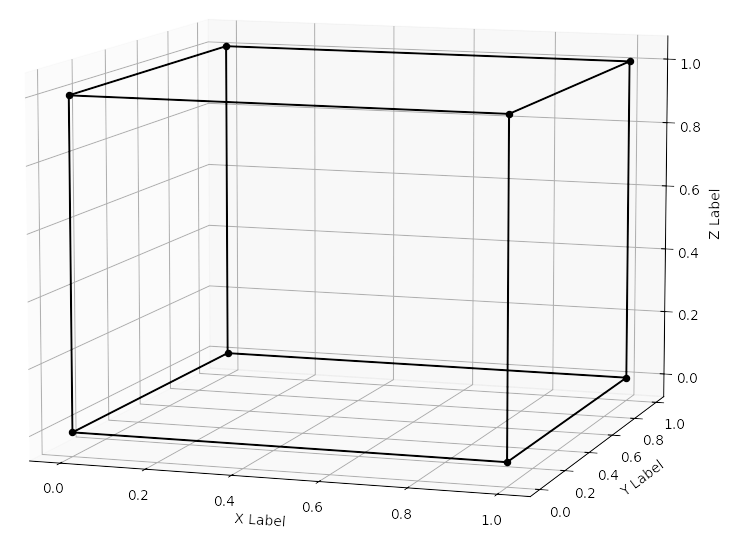
\includegraphics[width=0.7\linewidth]{images/ExampleCube.png}
	\caption{Расчетная область для кубика}
	\label{fig:ExampleCube}
\end{figure}

Попробуем подробить расчётную область (\ref{fig:ExampleCube}) на несколько частей. Получим сетку изображённую на рисунке (\ref{fig:GridCube}).

\begin{figure}
	\centering
	\vspace*{0.7cm}
	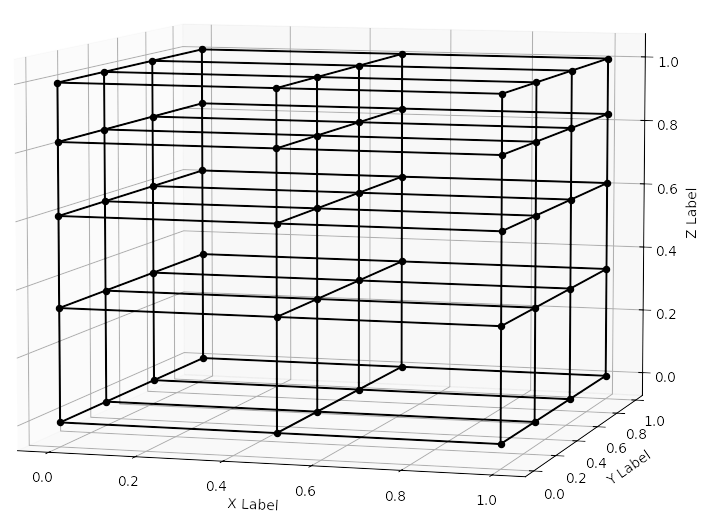
\includegraphics[width=0.7\linewidth]{images/GridCube.png}
	\caption{Секта для кубика}
	\label{fig:GridCube}
\end{figure}

Приведём ещё насколько примеров для построения сеток на шестигранниках, изображённых на рисунках  \ref{fig:Emerald} - \ref{fig:DEmerald}.

\begin{figure}
	\begin{minipage}[h]{0.49\linewidth}
		\center{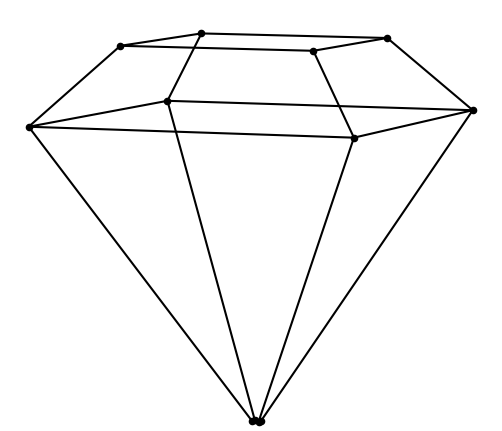
\includegraphics[width=0.5\linewidth]{images/EmeraldField.png} \\ а)}
	\end{minipage}
	\hfill
	\begin{minipage}[h]{0.49\linewidth}
		\center{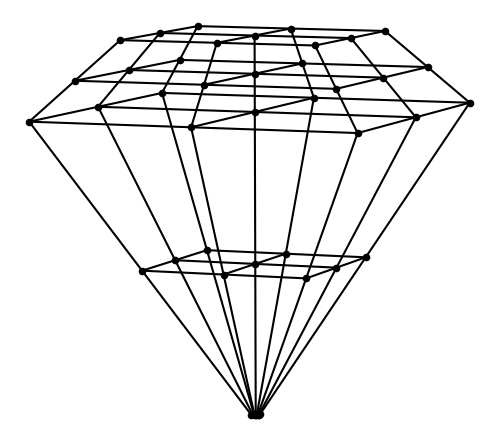
\includegraphics[width=0.5\linewidth]{images/EmeraldMesh.png} \\ б)}
	\end{minipage}
	\caption{Расчётная область в форме изумруда (а) и сетка к ней (б).}
	\label{fig:Emerald}
\end{figure}

\begin{figure}
	\begin{minipage}[h]{0.49\linewidth}
		\center{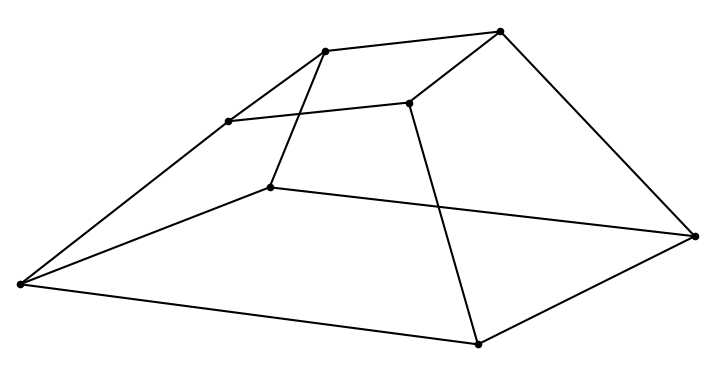
\includegraphics[width=0.5\linewidth]{images/PyramidField.png} \\ а)}
	\end{minipage}
	\hfill
	\begin{minipage}[h]{0.49\linewidth}
		\center{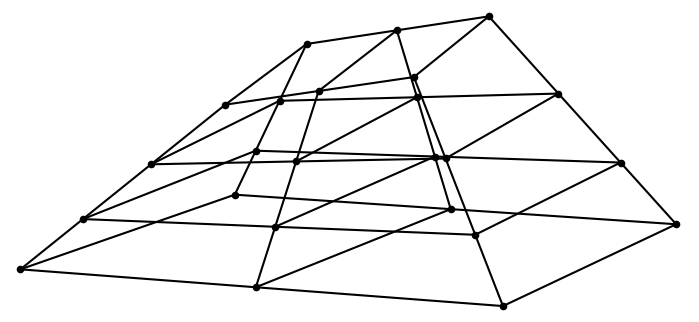
\includegraphics[width=0.5\linewidth]{images/PyramidMesh.png} \\ б)}
	\end{minipage}
	\caption{Расчётная область в форме скошенной пирамиды (а) и сетка к ней (б).}
	\label{fig:Pyramid}
\end{figure}

\begin{figure}
	\begin{minipage}[h]{0.49\linewidth}
		\center{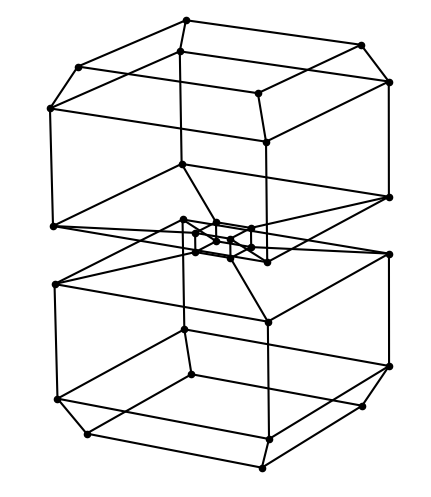
\includegraphics[width=0.5\linewidth]{images/HGField.png} \\ а)}
	\end{minipage}
	\hfill
	\begin{minipage}[h]{0.49\linewidth}
		\center{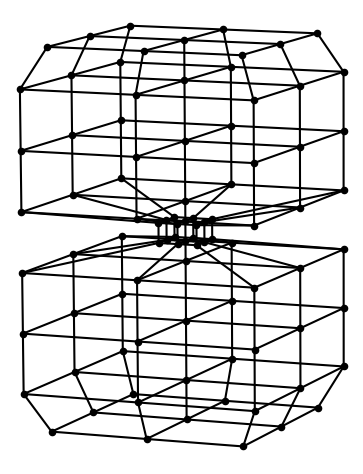
\includegraphics[width=0.5\linewidth]{images/HGMesh.png} \\ б)}
	\end{minipage}
	\caption{Расчётная область в форме песочных часов (а) и сетка к ней (б).}
	\label{fig:HG}
\end{figure}

\begin{figure}
	\begin{minipage}[h]{0.49\linewidth}
		\center{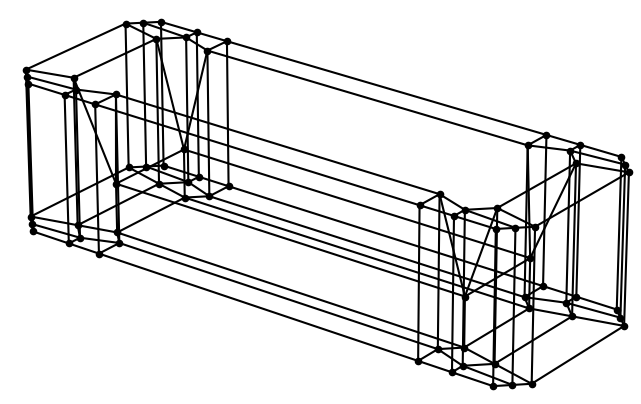
\includegraphics[width=0.5\linewidth]{images/BathField.png} \\ а)}
	\end{minipage}
	\hfill
	\begin{minipage}[h]{0.49\linewidth}
		\center{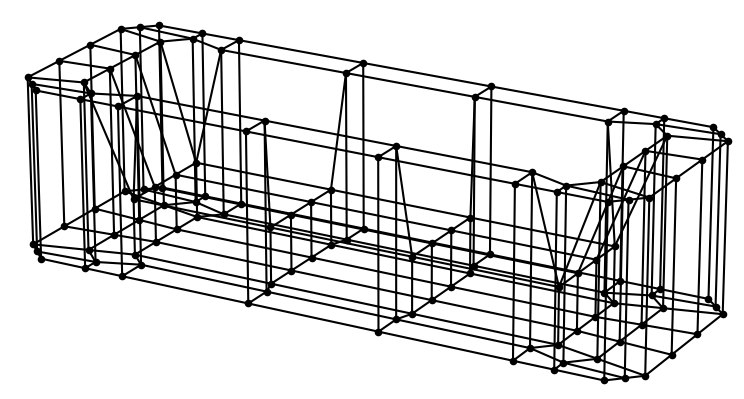
\includegraphics[width=0.5\linewidth]{images/BathMesh.png} \\ б)}
	\end{minipage}
	\caption{Расчётная область в форме ванной (а) и сетка к ней (б).}
	\label{fig:Bath}
\end{figure}

\begin{figure}
	\begin{minipage}[h]{0.49\linewidth}
		\center{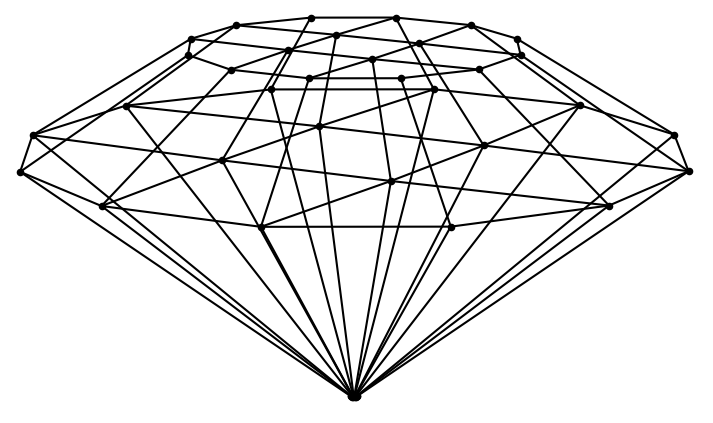
\includegraphics[width=0.5\linewidth]{images/DEmeraldField.png} \\ а)}
	\end{minipage}
	\hfill
	\begin{minipage}[h]{0.49\linewidth}
		\center{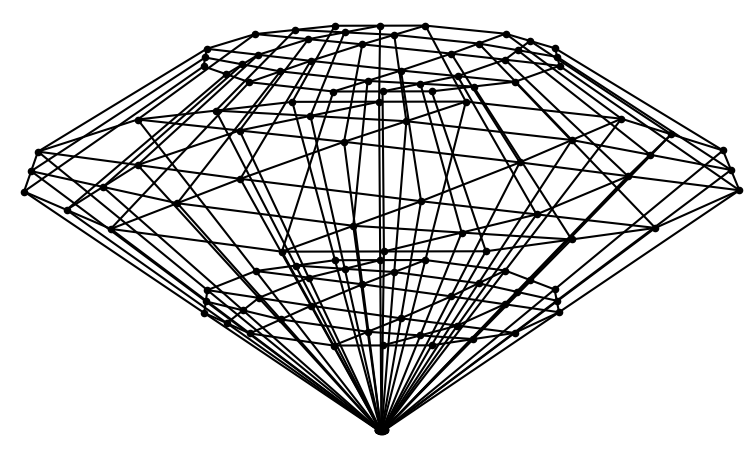
\includegraphics[width=0.5\linewidth]{images/DEmeraldMesh.png} \\ б)}
	\end{minipage}
	\caption{Расчётная область в форме детализированного изумруда (а) и сетка к ней (б).}
	\label{fig:DEmerald}
\end{figure}

Таким образом, программа для построения сетки может строить достаточно геометрически сложные фигуры.

\section{Численное интегрирование}

При расчёте элементов локальных матриц жёсткости (\ref{eq_1_11}) и масс (\ref{eq_1_12}) будем использовать численное интегрирование методами Гаусса разных порядков (2, 3, 4, 5). Результаты численного интегрирования на некоторых функциях приведены в таблицах \ref{tab:numIntegr1} - \ref{tab:numIntegr7}. Область интегрирования для всех функций единый: $\Omega_E \in \left[-1; 1\right]_x \cross \left[-1; 1\right]_y \cross \left[-1; 1\right]_z$.

\begin{table}
	\caption{Тестирование численного интегрирования на функции $u = 2$.}
	\centering
	\small
	\begin{tabularx}{1.0\textwidth}{| >{\raggedright\arraybackslash}X | >{\raggedright\arraybackslash}X | >{\raggedright\arraybackslash}X |>{\raggedright\arraybackslash}X |>{\raggedright\arraybackslash}X |}
		\hline
		\centering{Аналитический результат} & \centering{Гаусс 2} & \centering{Гаусс 3} & \centering{Гаусс 4} & \centering{Гаусс 5} \tabularnewline \hline
		
		\centering{16.0} & \centering{1.6000000e+01}& \centering{1.6000000e+01} & \centering{1.6000000e+01} & \centering{1.6000000e+01} \tabularnewline \hline
		
	\end{tabularx}
	\label{tab:numIntegr1}
\end{table}


\begin{table}
	\caption{Тестирование численного интегрирования на функции $u = x + y + z$.}
	\centering
	\small
	\begin{tabularx}{1.0\textwidth}{| >{\raggedright\arraybackslash}X | >{\raggedright\arraybackslash}X | >{\raggedright\arraybackslash}X |>{\raggedright\arraybackslash}X |>{\raggedright\arraybackslash}X |}
		\hline
		\centering{Аналитический результат} & \centering{Гаусс 2} & \centering{Гаусс 3} & \centering{Гаусс 4} & \centering{Гаусс 5} \tabularnewline \hline
		
		\centering{0.0} & \centering{0.0000000e+00}& \centering{-2.2204460e-16} & \centering{5.6898930e-16} & \centering{-6.5225603e-16} \tabularnewline \hline
		
	\end{tabularx}
	\label{tab:numIntegr2}
\end{table}

\begin{table}
	\caption{Тестирование численного интегрирования на функции $u = x^2 + y^2 + z^2$.}
	\centering
	\small
	\begin{tabularx}{1.0\textwidth}{| >{\raggedright\arraybackslash}X | >{\raggedright\arraybackslash}X | >{\raggedright\arraybackslash}X |>{\raggedright\arraybackslash}X |>{\raggedright\arraybackslash}X |}
		\hline
		\centering{Аналитический результат} & \centering{Гаусс 2} & \centering{Гаусс 3} & \centering{Гаусс 4} & \centering{Гаусс 5} \tabularnewline \hline
		
		\centering{8.0} & \centering{8.0000000e+00}& \centering{8.0000000e+00} & \centering{8.0000000e+00} & \centering{8.0000000e+00} \tabularnewline \hline
		
	\end{tabularx}
	\label{tab:numIntegr3}
\end{table}

\begin{table}
	\caption{Тестирование численного интегрирования на функции $u = x \cdot y \cdot z$.}
	\centering
	\small
	\begin{tabularx}{1.0\textwidth}{| >{\raggedright\arraybackslash}X | >{\raggedright\arraybackslash}X | >{\raggedright\arraybackslash}X |>{\raggedright\arraybackslash}X |>{\raggedright\arraybackslash}X |}
		\hline
		\centering{Аналитический результат} & \centering{Гаусс 2} & \centering{Гаусс 3} & \centering{Гаусс 4} & \centering{Гаусс 5} \tabularnewline \hline
		
		\centering{0.0} & \centering{8.0000000e+00}& \centering{0.0000000e+00} & \centering{0.0000000e+00} & \centering{8.6736174e-18} \tabularnewline \hline
		
	\end{tabularx}
	\label{tab:numIntegr4}
\end{table}

\begin{table}
	\caption{Тестирование численного интегрирования на функции $u = x^2 \cdot y^2 \cdot z^2$.}
	\centering
	\small
	\begin{tabularx}{1.0\textwidth}{| >{\raggedright\arraybackslash}X | >{\raggedright\arraybackslash}X | >{\raggedright\arraybackslash}X |>{\raggedright\arraybackslash}X |>{\raggedright\arraybackslash}X |}
		\hline
		\centering{Аналитический результат} & \centering{Гаусс 2} & \centering{Гаусс 3} & \centering{Гаусс 4} & \centering{Гаусс 5} \tabularnewline \hline
		
		\centering{$\frac{8}{27}$ $\approx$ 0.29630} & \centering{2.9629630e-01}& \centering{2.9629630e-01} & \centering{2.9629630e-01} & \centering{2.9629630e-01} \tabularnewline \hline
		
	\end{tabularx}
	\label{tab:numIntegr5}
\end{table}

\begin{table}
	\caption{Тестирование численного интегрирования на функции $u = \text{cos}(x + y + z)$.}
	\centering
	\small
	\begin{tabularx}{1.0\textwidth}{| >{\raggedright\arraybackslash}X | >{\raggedright\arraybackslash}X | >{\raggedright\arraybackslash}X |>{\raggedright\arraybackslash}X |>{\raggedright\arraybackslash}X |}
		\hline
		\centering{Аналитический результат} & \centering{Гаусс 2} & \centering{Гаусс 3} & \centering{Гаусс 4} & \centering{Гаусс 5} \tabularnewline \hline
		
		\centering{4.7666...} & \centering{4.7063579e+00}& \centering{4.7671091e+00} & \centering{4.7665835e+00} & \centering{4.7665859e+00} \tabularnewline \hline
		
	\end{tabularx}
	\label{tab:numIntegr6}
\end{table}

\begin{table}
	\caption{Тестирование численного интегрирования на функции $u = e^{x + y + z}$.}
	\centering
	\small
	\begin{tabularx}{1.0\textwidth}{| >{\raggedright\arraybackslash}X | >{\raggedright\arraybackslash}X | >{\raggedright\arraybackslash}X |>{\raggedright\arraybackslash}X |>{\raggedright\arraybackslash}X |}
		\hline
		\centering{Аналитический результат} & \centering{Гаусс 2} & \centering{Гаусс 3} & \centering{Гаусс 4} & \centering{Гаусс 5} \tabularnewline \hline
		
		\centering{12.9845...} & \centering{1.2857243e+01}& \centering{1.2983458e+01} & \centering{1.2984538e+01} & \centering{1.2984543e+01} \tabularnewline \hline
		
	\end{tabularx}
	\label{tab:numIntegr7}
\end{table}

\section{Решение СЛАУ}

Через LOS или Pardiso.

\section{Тестирование трёхмерной задачи на полиномиальных вектор-функциях}

Проведем сначала тестирование разработанной программы по векторному МКЭ на работоспособность. Образец расчетной области изображен на рисунке \ref{fig:exampleOfArea}. Это область $\Omega = [0.0, 3.0]_x \times [0.0, 3.0]_y \times [0.0, 3.0]_z$, она содержит 144 ребра, на всех границах будем задавать первые краевые условия. 

Тестирование будем проводить дифференциального уравнения (\ref{eq_4_2}):

\begin{equation} \label{eq_4_2}
	\text{rot} \left(\frac{1}{\mu} \text{rot} \overrightarrow{\textbf{A}}\right) + \gamma \overrightarrow{\textbf{A}} + \sigma \frac{\partial \overrightarrow{\textbf{A}}}{\partial t} = \overrightarrow{\textbf{F}}.
\end{equation}

В таблицах \ref{tab:test1} -- \ref{tab:test9} приведено тестирование на работоспособность программы.

\begin{table}
	\caption{Тестирование при $\overrightarrow{\textbf{A}} = (1.0, 1.0, 1.0)^{\text{T}}$, $\overrightarrow{\textbf{F}} = (1.0, 1.0, 1.0)^{\text{T}}$, $\mu = 1$, $\gamma = 1$, $\sigma = 0$}
	\centering
	\small
	\begin{tabularx}{1.0\textwidth}{| >{\raggedright\arraybackslash}X | >{\raggedright\arraybackslash}X | >{\raggedright\arraybackslash}X |>{\raggedright\arraybackslash}X |}
		\hline
		\centering{Ребро} & \centering{Значение} & \centering{Абсолютная погрешность} & \centering{Относительная погрешность} \tabularnewline \hline
		
		
		\centering{($x; 1.0; 1.0$)} & \centering{1.00000000E+000}& \centering{0.00000000E+000} & \centering{0.00000000E+000} \tabularnewline \hline
		
		\centering{($x; 2.0; 1.0$)} & \centering{1.00000000E+000}& \centering{0.00000000E+000} & \centering{0.00000000E+000} \tabularnewline \hline
		
		\centering{($x; 1.0; 2.0$)} & \centering{1.00000000E+000}& \centering{0.00000000E+000} & \centering{0.00000000E+000} \tabularnewline \hline
		
		\centering{($x; 2.0; 2.0$)} & \centering{1.00000000E+000}& \centering{0.00000000E+000} & \centering{0.00000000E+000} \tabularnewline \hline
		
		
		
		\centering{($1.0; y; 1.0$)} & \centering{1.00000000E+000}& \centering{0.00000000E+000} & \centering{0.00000000E+000} \tabularnewline \hline
		
		\centering{($2.0; y; 1.0$)} & \centering{1.00000000E+000}& \centering{0.00000000E+000} & \centering{0.00000000E+000} \tabularnewline \hline
		
		\centering{($1.0; y; 2.0$)} & \centering{1.00000000E+000}& \centering{0.00000000E+000} & \centering{0.00000000E+000} \tabularnewline \hline
		
		\centering{($2.0; y; 2.0$)} & \centering{1.00000000E+000}& \centering{0.00000000E+000} & \centering{0.00000000E+000} \tabularnewline \hline
		
		
		
		\centering{($1.0; 1.0; z$)} & \centering{1.00000000E+000}& \centering{0.00000000E+000} & \centering{0.00000000E+000} \tabularnewline \hline
		
		\centering{($2.0; 1.0; z$)} & \centering{1.00000000E+000}& \centering{0.00000000E+000} & \centering{0.00000000E+000} \tabularnewline \hline
		
		\centering{($1.0; 2.0; z$)} & \centering{1.00000000E+000}& \centering{0.00000000E+000} & \centering{0.00000000E+000} \tabularnewline \hline
		
		\centering{($2.0; 2.0; z$)} & \centering{1.00000000E+000}& \centering{0.00000000E+000} & \centering{0.00000000E+000} \tabularnewline \hline
		
		
	\end{tabularx}
	\label{tab:test1}
\end{table}

\begin{table}
	\caption{Тестирование при $\overrightarrow{\textbf{A}} = (y, z, x)^{\text{T}}$, $\overrightarrow{\textbf{F}} = (y, z, x)^{\text{T}}$, $\mu = 1$, $\gamma = 1$, $\sigma = 0$}
	\centering
	\small
	\begin{tabularx}{1.0\textwidth}{| >{\raggedright\arraybackslash}X | >{\raggedright\arraybackslash}X | >{\raggedright\arraybackslash}X |>{\raggedright\arraybackslash}X |}
		\hline
		\centering{Ребро} & \centering{Значение} & \centering{Абсолютная погрешность} & \centering{Относительная погрешность} \tabularnewline \hline
		
		\centering{($x; 1.0; 1.0$)} & \centering{1.00000000E+000}& \centering{0.00000000E+000} & \centering{0.00000000E+000} \tabularnewline \hline
		
		\centering{($x; 2.0; 1.0$)} & \centering{2.00000000E+000}& \centering{0.00000000E+000} & \centering{0.00000000E+000} \tabularnewline \hline
		
		\centering{($x; 1.0; 2.0$)} & \centering{1.00000000E+000}& \centering{0.00000000E+000} & \centering{0.00000000E+000} \tabularnewline \hline
		
		\centering{($x; 2.0; 2.0$)} & \centering{2.00000000E+000}& \centering{0.00000000E+000} & \centering{0.00000000E+000} \tabularnewline \hline
		
		
		
		\centering{($1.0; y; 1.0$)} & \centering{1.00000000E+000}& \centering{0.00000000E+000} & \centering{0.00000000E+000} \tabularnewline \hline
		
		\centering{($2.0; y; 1.0$)} & \centering{1.00000000E+000}& \centering{0.00000000E+000} & \centering{0.00000000E+000} \tabularnewline \hline
		
		\centering{($1.0; y; 2.0$)} & \centering{2.00000000E+000}& \centering{0.00000000E+000} & \centering{0.00000000E+000} \tabularnewline \hline
		
		\centering{($2.0; y; 2.0$)} & \centering{2.00000000E+000}& \centering{0.00000000E+000} & \centering{0.00000000E+000} \tabularnewline \hline
		
		
		
		\centering{($1.0; 1.0; z$)} & \centering{1.00000000E+000}& \centering{0.00000000E+000} & \centering{0.00000000E+000} \tabularnewline \hline
		
		\centering{($2.0; 1.0; z$)} & \centering{2.00000000E+000}& \centering{0.00000000E+000} & \centering{0.00000000E+000} \tabularnewline \hline
		
		\centering{($1.0; 2.0; z$)} & \centering{1.00000000E+000}& \centering{0.00000000E+000} & \centering{0.00000000E+000} \tabularnewline \hline
		
		\centering{($2.0; 2.0; z$)} & \centering{2.00000000E+000}& \centering{0.00000000E+000} & \centering{0.00000000E+000} \tabularnewline \hline
		
		
	\end{tabularx}
	\label{tab:test2}
\end{table}

\begin{table}
	\caption{Тестирование при $\overrightarrow{\textbf{A}} = (1 + y + x; 1 + x + z; 1 + x + y)^{\text{T}}$, $\overrightarrow{\textbf{F}} = (1 + y + x; 1 + x + z; 1 + x + y)^{\text{T}}$, $\mu = 1$, $\gamma = 1$, $\sigma = 0$}
	\centering
	\small
	\begin{tabularx}{1.0\textwidth}{| >{\raggedright\arraybackslash}X | >{\raggedright\arraybackslash}X | >{\raggedright\arraybackslash}X |>{\raggedright\arraybackslash}X |}
		\hline
		\centering{Ребро} & \centering{Значение} & \centering{Абсолютная погрешность} & \centering{Относительная погрешность} \tabularnewline \hline
		
		
		\centering{($x; 1.0; 1.0$)} & \centering{3.00000000E+000}& \centering{0.00000000E+000} & \centering{0.00000000E+000} \tabularnewline \hline
		
		\centering{($x; 2.0; 1.0$)} & \centering{4.00000000E+000}& \centering{0.00000000E+000} & \centering{0.00000000E+000} \tabularnewline \hline
		
		\centering{($x; 1.0; 2.0$)} & \centering{4.00000000E+000}& \centering{0.00000000E+000} & \centering{0.00000000E+000} \tabularnewline \hline
		
		\centering{($x; 2.0; 2.0$)} & \centering{5.00000000E+000}& \centering{0.00000000E+000} & \centering{0.00000000E+000} \tabularnewline \hline
		
		
		
		\centering{($1.0; y; 1.0$)} & \centering{3.00000000E+000}& \centering{0.00000000E+000} & \centering{0.00000000E+000} \tabularnewline \hline
		
		\centering{($2.0; y; 1.0$)} & \centering{4.00000000E+000}& \centering{0.00000000E+000} & \centering{0.00000000E+000} \tabularnewline \hline
		
		\centering{($1.0; y; 2.0$)} & \centering{4.00000000E+000}& \centering{0.00000000E+000} & \centering{0.00000000E+000} \tabularnewline \hline
		
		\centering{($2.0; y; 2.0$)} & \centering{5.00000000E+000}& \centering{0.00000000E+000} & \centering{0.00000000E+000} \tabularnewline \hline
		
		
		
		\centering{($1.0; 1.0; z$)} & \centering{3.00000000E+000}& \centering{0.00000000E+000} & \centering{0.00000000E+000} \tabularnewline \hline
		
		\centering{($2.0; 1.0; z$)} & \centering{4.00000000E+000}& \centering{0.00000000E+000} & \centering{0.00000000E+000} \tabularnewline \hline
		
		\centering{($1.0; 2.0; z$)} & \centering{4.00000000E+000}& \centering{0.00000000E+000} & \centering{0.00000000E+000} \tabularnewline \hline
		
		\centering{($2.0; 2.0; z$)} & \centering{5.00000000E+000}& \centering{0.00000000E+000} & \centering{0.00000000E+000} \tabularnewline \hline
		
	\end{tabularx}
	\label{tab:test3}
\end{table}

\begin{table}
	\caption{Тестирование при $\overrightarrow{\textbf{A}} = (y - z; x - z; x - y)^{\text{T}}$, $\overrightarrow{\textbf{F}} = (y - x; x - z; x - y)^{\text{T}}$, $\mu = 1$, $\gamma = 1$, $\sigma = 0$}
	\centering
	\small
	\begin{tabularx}{1.0\textwidth}{| >{\raggedright\arraybackslash}X | >{\raggedright\arraybackslash}X | >{\raggedright\arraybackslash}X |>{\raggedright\arraybackslash}X |}
		\hline
		\centering{Ребро} & \centering{Значение} & \centering{Абсолютная погрешность} & \centering{Относительная погрешность} \tabularnewline \hline
		
		
		\centering{($x; 1.0; 1.0$)} & \centering{2.35132600E-016}& \centering{2.35132600E-016} & \centering{0.00000000E+000} \tabularnewline \hline
		
		\centering{($x; 2.0; 1.0$)} & \centering{1.00000000E+000}& \centering{0.00000000E+000} & \centering{0.00000000E+000} \tabularnewline \hline
		
		\centering{($x; 1.0; 2.0$)} & \centering{-1.00000000E+000}& \centering{0.00000000E+000} & \centering{0.00000000E+000} \tabularnewline \hline
		
		\centering{($x; 2.0; 2.0$)} & \centering{-5.55111512E-016}& \centering{-5.55111512E-016} & \centering{0.00000000E+000} \tabularnewline \hline
		
		
		
		\centering{($1.0; y; 1.0$)} & \centering{-3.97378607E-016}& \centering{-3.97378607E-016} & \centering{0.00000000E+000} \tabularnewline \hline
		
		\centering{($2.0; y; 1.0$)} & \centering{1.00000000E+000}& \centering{0.00000000E+000} & \centering{0.00000000E+000} \tabularnewline \hline
		
		\centering{($1.0; y; 2.0$)} & \centering{-1.00000000E+000}& \centering{0.00000000E+000} & \centering{0.00000000E+000} \tabularnewline \hline
		
		\centering{($2.0; y; 2.0$)} & \centering{-1.94289029E-016}& \centering{-1.94289029E-016} & \centering{0.00000000E+000} \tabularnewline \hline
		
		
		
		\centering{($1.0; 1.0; z$)} & \centering{-2.74847895E-016}& \centering{-2.74847895E-016} & \centering{0.00000000E+000} \tabularnewline \hline
		
		\centering{($2.0; 1.0; z$)} & \centering{1.00000000E+000}& \centering{0.00000000E+000} & \centering{0.00000000E+000} \tabularnewline \hline
		
		\centering{($1.0; 2.0; z$)} & \centering{-1.00000000E+000}& \centering{0.00000000E+000} & \centering{0.00000000E+000} \tabularnewline \hline
		
		\centering{($2.0; 2.0; z$)} & \centering{4.27842044E-016}& \centering{4.27842044E-016} & \centering{0.00000000E+000} \tabularnewline \hline
		
		
	\end{tabularx}
	\label{tab:test4}
\end{table}

\begin{table}
	\caption{Тестирование при $\overrightarrow{\textbf{A}} = (y \cdot z; x \cdot z; x \cdot y)^{\text{T}}$, $\overrightarrow{\textbf{F}} = (y \cdot z; x \cdot z; x \cdot y)^{\text{T}}$, $\mu = 1$, $\gamma = 1$, $\sigma = 0$}
	\centering
	\small
	\begin{tabularx}{1.0\textwidth}{| >{\raggedright\arraybackslash}X | >{\raggedright\arraybackslash}X | >{\raggedright\arraybackslash}X |>{\raggedright\arraybackslash}X |}
		\hline
		\centering{Ребро} & \centering{Значение} & \centering{Абсолютная погрешность} & \centering{Относительная погрешность} \tabularnewline \hline
		
		
		\centering{($x; 1.0; 1.0$)} & \centering{1.00000000E+000}& \centering{0.00000000E+000} & \centering{0.00000000E+000} \tabularnewline \hline
		
		\centering{($x; 2.0; 1.0$)} & \centering{2.00000000E+000}& \centering{0.00000000E+000} & \centering{0.00000000E+000} \tabularnewline \hline
		
		\centering{($x; 1.0; 2.0$)} & \centering{2.00000000E+000}& \centering{0.00000000E+000} & \centering{0.00000000E+000} \tabularnewline \hline
		
		\centering{($x; 2.0; 2.0$)} & \centering{4.00000000E+000}& \centering{0.00000000E+000} & \centering{0.00000000E+000} \tabularnewline \hline
		
		
		
		\centering{($1.0; y; 1.0$)} & \centering{1.00000000E+000}& \centering{0.00000000E+000} & \centering{0.00000000E+000} \tabularnewline \hline
		
		\centering{($2.0; y; 1.0$)} & \centering{2.00000000E+000}& \centering{0.00000000E+000} & \centering{0.00000000E+000} \tabularnewline \hline
		
		\centering{($1.0; y; 2.0$)} & \centering{2.00000000E+000}& \centering{0.00000000E+000} & \centering{0.00000000E+000} \tabularnewline \hline
		
		\centering{($2.0; y; 2.0$)} & \centering{4.00000000E+000}& \centering{0.00000000E+000} & \centering{0.00000000E+000} \tabularnewline \hline
		
		\centering{($1.0; 1.0; z$)} & \centering{1.00000000E+000}& \centering{0.00000000E+000} & \centering{0.00000000E+000} \tabularnewline \hline
		
		\centering{($2.0; 1.0; z$)} & \centering{2.00000000E+000}& \centering{0.00000000E+000} & \centering{0.00000000E+000} \tabularnewline \hline
		
		\centering{($1.0; 2.0; z$)} & \centering{2.00000000E+000}& \centering{0.00000000E+000} & \centering{0.00000000E+000} \tabularnewline \hline
		
		\centering{($2.0; 2.0; z$)} & \centering{4.00000000E+000}& \centering{0.00000000E+000} & \centering{0.00000000E+000} \tabularnewline \hline
		
	\end{tabularx}
	\label{tab:test5}
\end{table}

\begin{table}
	\caption{Тестирование при $\overrightarrow{\textbf{A}} = (y^2; z^2; x^2)^{\text{T}}$, $\overrightarrow{\textbf{F}} = (y^2 - 2; z^2 - 2; x^2 - 2)^{\text{T}}$, $\mu = 1$, $\gamma = 1$, $\sigma = 0$}
	\centering
	\small
	\begin{tabularx}{1.0\textwidth}{| >{\raggedright\arraybackslash}X | >{\raggedright\arraybackslash}X | >{\raggedright\arraybackslash}X |>{\raggedright\arraybackslash}X |}
		\hline
		\centering{Ребро} & \centering{Значение} & \centering{Абсолютная погрешность} & \centering{Относительная погрешность} \tabularnewline \hline
		
		
		\centering{($x; 1.0; 1.0$)} & \centering{1.00000000E+000}& \centering{0.00000000E+000} & \centering{0.00000000E+000} \tabularnewline \hline
		
		\centering{($x; 2.0; 1.0$)} & \centering{4.00000000E+000}& \centering{0.00000000E+000} & \centering{0.00000000E+000} \tabularnewline \hline
		
		\centering{($x; 1.0; 2.0$)} & \centering{1.00000000E+000}& \centering{0.00000000E+000} & \centering{0.00000000E+000} \tabularnewline \hline
		
		\centering{($x; 2.0; 2.0$)} & \centering{4.00000000E+000}& \centering{0.00000000E+000} & \centering{0.00000000E+000} \tabularnewline \hline
		
		
		
		\centering{($1.0; y; 1.0$)} & \centering{1.00000000E+000}& \centering{0.00000000E+000} & \centering{0.00000000E+000} \tabularnewline \hline
		
		\centering{($2.0; y; 1.0$)} & \centering{1.00000000E+000}& \centering{0.00000000E+000} & \centering{0.00000000E+000} \tabularnewline \hline
		
		\centering{($1.0; y; 2.0$)} & \centering{4.00000000E+000}& \centering{0.00000000E+000} & \centering{0.00000000E+000} \tabularnewline \hline
		
		\centering{($2.0; y; 2.0$)} & \centering{4.00000000E+000}& \centering{0.00000000E+000} & \centering{0.00000000E+000} \tabularnewline \hline
		
		
		
		\centering{($1.0; 1.0; z$)} & \centering{1.00000000E+000}& \centering{0.00000000E+000} & \centering{0.00000000E+000} \tabularnewline \hline
		
		\centering{($2.0; 1.0; z$)} & \centering{4.00000000E+000}& \centering{0.00000000E+000} & \centering{0.00000000E+000} \tabularnewline \hline
		
		\centering{($1.0; 2.0; z$)} & \centering{1.00000000E+000}& \centering{0.00000000E+000} & \centering{0.00000000E+000} \tabularnewline \hline
		
		\centering{($2.0; 2.0; z$)} & \centering{4.00000000E+000}& \centering{0.00000000E+000} & \centering{0.00000000E+000} \tabularnewline \hline
	\end{tabularx}
	\label{tab:test6}
\end{table}

\begin{table}
	\caption{Тестирование при $\overrightarrow{\textbf{A}} = (y^2 + z^2; x^2 + z^2; x^2 + y^2)^{\text{T}}$, $\overrightarrow{\textbf{F}} = (y^2 + z^2 - 4; x^2 + z^2 - 4; x^2 + y^2 - 4)^{\text{T}}$, $\mu = 1$, $\gamma = 1$, $\sigma = 0$}
	\centering
	\small
	\begin{tabularx}{1.0\textwidth}{| >{\raggedright\arraybackslash}X | >{\raggedright\arraybackslash}X | >{\raggedright\arraybackslash}X |>{\raggedright\arraybackslash}X |}
		\hline
		\centering{Ребро} & \centering{Значение} & \centering{Абсолютная погрешность} & \centering{Относительная погрешность} \tabularnewline \hline
		
		
		\centering{($x; 1.0; 1.0$)} & \centering{2.00000000E+000}& \centering{0.00000000E+000} & \centering{0.00000000E+000} \tabularnewline \hline
		
		\centering{($x; 2.0; 1.0$)} & \centering{5.00000000E+000}& \centering{0.00000000E+000} & \centering{0.00000000E+000} \tabularnewline \hline
		
		\centering{($x; 1.0; 2.0$)} & \centering{5.00000000E+000}& \centering{0.00000000E+000} & \centering{0.00000000E+000} \tabularnewline \hline
		
		\centering{($x; 2.0; 2.0$)} & \centering{8.00000000E+000}& \centering{0.00000000E+000} & \centering{0.00000000E+000} \tabularnewline \hline
		
		
		
		\centering{($1.0; y; 1.0$)} & \centering{2.00000000E+000}& \centering{0.00000000E+000} & \centering{0.00000000E+000} \tabularnewline \hline
		
		\centering{($2.0; y; 1.0$)} & \centering{5.00000000E+000}& \centering{0.00000000E+000} & \centering{0.00000000E+000} \tabularnewline \hline
		
		\centering{($1.0; y; 2.0$)} & \centering{5.00000000E+000}& \centering{0.00000000E+000} & \centering{0.00000000E+000} \tabularnewline \hline
		
		\centering{($2.0; y; 2.0$)} & \centering{8.00000000E+000}& \centering{0.00000000E+000} & \centering{0.00000000E+000} \tabularnewline \hline
		
		
		
		\centering{($1.0; 1.0; z$)} & \centering{2.00000000E+000}& \centering{0.00000000E+000} & \centering{0.00000000E+000} \tabularnewline \hline
		
		\centering{($2.0; 1.0; z$)} & \centering{5.00000000E+000}& \centering{0.00000000E+000} & \centering{0.00000000E+000} \tabularnewline \hline
		
		\centering{($1.0; 2.0; z$)} & \centering{5.00000000E+000}& \centering{0.00000000E+000} & \centering{0.00000000E+000} \tabularnewline \hline
		
		\centering{($2.0; 2.0; z$)} & \centering{8.00000000E+000}& \centering{0.00000000E+000} & \centering{0.00000000E+000} \tabularnewline \hline
		
	\end{tabularx}
	\label{tab:test7}
\end{table}

\begin{table}
	\caption{Тестирование при $\overrightarrow{\textbf{A}} = (y^3; 0; 0)^{\text{T}}$, $\overrightarrow{\textbf{F}} = (y^3 - 6y; 0; 0)^{\text{T}}$, $\mu = 1$, $\gamma = 1$, $\sigma = 0$}
	\centering
	\small
	\begin{tabularx}{1.0\textwidth}{| >{\raggedright\arraybackslash}X | >{\raggedright\arraybackslash}X | >{\raggedright\arraybackslash}X |>{\raggedright\arraybackslash}X |}
		\hline
		\centering{Ребро} & \centering{Значение} & \centering{Абсолютная погрешность} & \centering{Относительная погрешность} \tabularnewline \hline
		
		
		\centering{($x; 1.0; 1.0$)} & \centering{1.00000000E+000}& \centering{0.00000000E+000} & \centering{0.00000000E+000} \tabularnewline \hline
		
		\centering{($x; 2.0; 1.0$)} & \centering{8.00000000E+000}& \centering{0.00000000E+000} & \centering{0.00000000E+000} \tabularnewline \hline
		
		\centering{($x; 1.0; 2.0$)} & \centering{1.00000000E+000}& \centering{0.00000000E+000} & \centering{0.00000000E+000} \tabularnewline \hline
		
		\centering{($x; 2.0; 2.0$)} & \centering{8.00000000E+000}& \centering{0.00000000E+000} & \centering{0.00000000E+000} \tabularnewline \hline
		
		
		
		\centering{($1.0; y; 1.0$)} & \centering{0.00000000E+000}& \centering{0.00000000E+000} & \centering{0.00000000E+000} \tabularnewline \hline
		
		\centering{($2.0; y; 1.0$)} & \centering{0.00000000E+000}& \centering{0.00000000E+000} & \centering{0.00000000E+000} \tabularnewline \hline
		
		\centering{($1.0; y; 2.0$)} & \centering{0.00000000E+000}& \centering{0.00000000E+000} & \centering{0.00000000E+000} \tabularnewline \hline
		
		\centering{($2.0; y; 2.0$)} & \centering{0.00000000E+000}& \centering{0.00000000E+000} & \centering{0.00000000E+000} \tabularnewline \hline
		
		
		
		\centering{($1.0; 1.0; z$)} & \centering{0.00000000E+000}& \centering{0.00000000E+000} & \centering{0.00000000E+000} \tabularnewline \hline
		
		\centering{($2.0; 1.0; z$)} & \centering{0.00000000E+000}& \centering{0.00000000E+000} & \centering{0.00000000E+000} \tabularnewline \hline
		
		\centering{($1.0; 2.0; z$)} & \centering{0.00000000E+000}& \centering{0.00000000E+000} & \centering{0.00000000E+000} \tabularnewline \hline
		
		\centering{($2.0; 2.0; z$)} & \centering{0.00000000E+000}& \centering{0.00000000E+000} & \centering{0.00000000E+000} \tabularnewline \hline
		
	\end{tabularx}
	\label{tab:test8}
\end{table}

\begin{table}
	\caption{Тестирование при $\overrightarrow{\textbf{A}} = (y^2 \cdot z^2; x^2 \cdot z^2; x^2 \cdot y^2)^{\text{T}}$, $\overrightarrow{\textbf{F}} = (y^2 \cdot z^2 - 2(y^2 + z^2); x^2 \cdot z^2 - 2(x^2 + z^2); x^2 \cdot y^2 - 2(x^2 + y^2))^{\text{T}}$, $\mu = 1$, $\gamma = 1$, $\sigma = 0$}
	\centering
	\small
	\begin{tabularx}{1.0\textwidth}{| >{\raggedright\arraybackslash}X | >{\raggedright\arraybackslash}X | >{\raggedright\arraybackslash}X |>{\raggedright\arraybackslash}X |}
		\hline
		\centering{Ребро} & \centering{Значение} & \centering{Абсолютная погрешность} & \centering{Относительная погрешность} \tabularnewline \hline
		
		
		\centering{($x; 1.0; 1.0$)} & \centering{1.00000000E+000}& \centering{0.00000000E+000} & \centering{0.00000000E+000} \tabularnewline \hline
		
		\centering{($x; 2.0; 1.0$)} & \centering{4.00000000E+000}& \centering{0.00000000E+000} & \centering{0.00000000E+000} \tabularnewline \hline
		
		\centering{($x; 1.0; 2.0$)} & \centering{4.00000000E+000}& \centering{0.00000000E+000} & \centering{0.00000000E+000} \tabularnewline \hline
		
		\centering{($x; 2.0; 2.0$)} & \centering{1.60000000E+001}& \centering{0.00000000E+000} & \centering{0.00000000E+000} \tabularnewline \hline
		
		
		
		\centering{($1.0; y; 1.0$)} & \centering{1.00000000E+000}& \centering{0.00000000E+000} & \centering{0.00000000E+000} \tabularnewline \hline
		
		\centering{($2.0; y; 1.0$)} & \centering{4.00000000E+000}& \centering{0.00000000E+000} & \centering{0.00000000E+000} \tabularnewline \hline
		
		\centering{($1.0; y; 2.0$)} & \centering{4.00000000E+000}& \centering{0.00000000E+000} & \centering{0.00000000E+000} \tabularnewline \hline
		
		\centering{($2.0; y; 2.0$)} & \centering{1.60000000E+001}& \centering{0.00000000E+000} & \centering{0.00000000E+000} \tabularnewline \hline
		
		
		
		\centering{($1.0; 1.0; z$)} & \centering{1.00000000E+000}& \centering{0.00000000E+000} & \centering{0.00000000E+000} \tabularnewline \hline
		
		\centering{($2.0; 1.0; z$)} & \centering{4.00000000E+000}& \centering{0.00000000E+000} & \centering{0.00000000E+000} \tabularnewline \hline
		
		\centering{($1.0; 2.0; z$)} & \centering{4.00000000E+000}& \centering{0.00000000E+000} & \centering{0.00000000E+000} \tabularnewline \hline
		
		\centering{($2.0; 2.0; z$)} & \centering{1.60000000E+001}& \centering{0.00000000E+000} & \centering{0.00000000E+000} \tabularnewline \hline
		
	\end{tabularx}
	\label{tab:test9}
\end{table}

Проведём тестирование на порядок аппроксимации. Для оценки будем брать значения вектор-функции в центрах параллелепипедов. Сетка по пространству для данных тестов изображена на рисунке \ref{fig:exampleOfArea_1}.


В таблицах \ref{tab:test10} -- \ref{tab:test11} представлены результаты тестирования для постоянной и линейной вектор-функциях.

\begin{table}
	\caption{Тестирование при $\overrightarrow{\textbf{A}} = (1.0; 1.0; 1.0)^{\text{T}}$, $\overrightarrow{\textbf{F}} = (1.0; 1.0; 1.0)^{\text{T}}$, $\mu = 1$, $\gamma = 1$, $\sigma = 0$}
	\centering
	\small
	\begin{tabularx}{1.0\textwidth}{| >{\raggedright\arraybackslash}X | >{\raggedright\arraybackslash}X | >{\raggedright\arraybackslash}X |>{\raggedright\arraybackslash}X |}
		\hline
		\centering{Ребро} & \centering{Значение} & \centering{Абсолютная погрешность} & \centering{Относительная погрешность} \tabularnewline \hline
		
		
		\centering{($0.5; 0.5; 0.5$)} & \centering{1.00000000E+000 \\ 1.00000000E+000\\
			1.00000000E+000}& \centering{0.00000000E+000 \\ 0.00000000E+000 \\ 0.00000000E+000} & \centering{0.00000000E+000 \\ 0.00000000E+000 \\ 0.00000000E+000} \tabularnewline \hline
		
		\centering{($1.5; 0.5; 0.5$)} & \centering{1.00000000E+000 \\ 1.00000000E+000\\
			1.00000000E+000}& \centering{0.00000000E+000 \\ 0.00000000E+000 \\ 0.00000000E+000} & \centering{0.00000000E+000 \\ 0.00000000E+000 \\ 0.00000000E+000} \tabularnewline \hline
		
		\centering{($0.5; 1.5; 0.5$)} & \centering{1.00000000E+000 \\ 1.00000000E+000\\
			1.00000000E+000}& \centering{0.00000000E+000 \\ 0.00000000E+000 \\ 0.00000000E+000} & \centering{0.00000000E+000 \\ 0.00000000E+000 \\ 0.00000000E+000} \tabularnewline \hline
		
		\centering{($1.5; 1.5; 0.5$)} & \centering{1.00000000E+000 \\ 1.00000000E+000\\
			1.00000000E+000}& \centering{0.00000000E+000 \\ 0.00000000E+000 \\ 0.00000000E+000} & \centering{0.00000000E+000 \\ 0.00000000E+000 \\ 0.00000000E+000} \tabularnewline \hline
			
		\centering{($0.5; 0.5; 1.5$)} & \centering{1.00000000E+000 \\ 1.00000000E+000\\
			1.00000000E+000}& \centering{0.00000000E+000 \\ 0.00000000E+000 \\ 0.00000000E+000} & \centering{0.00000000E+000 \\ 0.00000000E+000 \\ 0.00000000E+000} \tabularnewline \hline
		
		\centering{($1.5; 0.5; 1.5$)} & \centering{1.00000000E+000 \\ 1.00000000E+000\\
			1.00000000E+000}& \centering{0.00000000E+000 \\ 0.00000000E+000 \\ 0.00000000E+000} & \centering{0.00000000E+000 \\ 0.00000000E+000 \\ 0.00000000E+000} \tabularnewline \hline
		
		\centering{($0.5; 1.5; 1.5$)} & \centering{1.00000000E+000 \\ 1.00000000E+000\\
			1.00000000E+000}& \centering{0.00000000E+000 \\ 0.00000000E+000 \\ 0.00000000E+000} & \centering{0.00000000E+000 \\ 0.00000000E+000 \\ 0.00000000E+000} \tabularnewline \hline
		
		\centering{($1.5; 1.5; 1.5$)} & \centering{1.00000000E+000 \\ 1.00000000E+000\\
			1.00000000E+000}& \centering{0.00000000E+000 \\ 0.00000000E+000 \\ 0.00000000E+000} & \centering{0.00000000E+000 \\ 0.00000000E+000 \\ 0.00000000E+000} \tabularnewline \hline
	
	\end{tabularx}
	\label{tab:test10}
\end{table}

\begin{table}
	\caption{Тестирование при $\overrightarrow{\textbf{A}} = (y; z; x)^{\text{T}}$, $\overrightarrow{\textbf{F}} = (y; z; x)^{\text{T}}$, $\mu = 1$, $\gamma = 1$, $\sigma = 0$}
	\centering
	\small
	\begin{tabularx}{1.0\textwidth}{| >{\raggedright\arraybackslash}X | >{\raggedright\arraybackslash}X | >{\raggedright\arraybackslash}X |>{\raggedright\arraybackslash}X |}
		\hline
		\centering{Ребро} & \centering{Значение} & \centering{Абсолютная погрешность} & \centering{Относительная погрешность} \tabularnewline \hline
		
		
		\centering{($0.5; 0.5; 0.5$)} & \centering{5.00000000E-001 \\ 5.00000000E-001 \\
			5.00000000E-001}& \centering{0.00000000E+000 \\ 0.00000000E+000 \\ 0.00000000E+000} & \centering{0.00000000E+000 \\ 0.00000000E+000 \\ 0.00000000E+000} \tabularnewline \hline
		
		\centering{($1.5; 0.5; 0.5$)} & \centering{5.00000000E-001 \\ 5.00000000E-001\\
			1.50000000E+000}& \centering{0.00000000E+000 \\ 0.00000000E+000 \\ 0.00000000E+000} & \centering{0.00000000E+000 \\ 0.00000000E+000 \\ 0.00000000E+000} \tabularnewline \hline
		
		\centering{($0.5; 1.5; 0.5$)} & \centering{1.50000000E+000 \\ 5.00000000E-001\\
			5.00000000E-001}& \centering{0.00000000E+000 \\ 0.00000000E+000 \\ 0.00000000E+000} & \centering{0.00000000E+000 \\ 0.00000000E+000 \\ 0.00000000E+000} \tabularnewline \hline
		
		\centering{($1.5; 1.5; 0.5$)} & \centering{1.50000000E+000 \\ 5.00000000E-001\\
			1.50000000E+000}& \centering{0.00000000E+000 \\ 0.00000000E+000 \\ 0.00000000E+000} & \centering{0.00000000E+000 \\ 0.00000000E+000 \\ 0.00000000E+000} \tabularnewline \hline
		
		\centering{($0.5; 0.5; 1.5$)} & \centering{5.00000000E-001 \\ 1.50000000E+000\\
			5.00000000E-001}& \centering{0.00000000E+000 \\ 0.00000000E+000 \\ 0.00000000E+000} & \centering{0.00000000E+000 \\ 0.00000000E+000 \\ 0.00000000E+000} \tabularnewline \hline
		
		\centering{($1.5; 0.5; 1.5$)} & \centering{5.00000000E-001 \\ 1.50000000E+000\\
			5.00000000E-001}& \centering{0.00000000E+000 \\ 0.00000000E+000 \\ 0.00000000E+000} & \centering{0.00000000E+000 \\ 0.00000000E+000 \\ 0.00000000E+000} \tabularnewline \hline
		
		\centering{($0.5; 1.5; 1.5$)} & \centering{1.50000000E+000 \\ 1.50000000E+000\\
			5.00000000E-001}& \centering{0.00000000E+000 \\ 0.00000000E+000 \\ 0.00000000E+000} & \centering{0.00000000E+000 \\ 0.00000000E+000 \\ 0.00000000E+000} \tabularnewline \hline
		
		\centering{($1.5; 1.5; 1.5$)} & \centering{1.50000000E+000 \\ 1.50000000E+000\\
			1.50000000E+000}& \centering{0.00000000E+000 \\ 0.00000000E+000 \\ 0.00000000E+000} & \centering{0.00000000E+000 \\ 0.00000000E+000 \\ 0.00000000E+000} \tabularnewline \hline
		
	\end{tabularx}
	\label{tab:test11}
\end{table}

Как и предполагали, при использовании билинейных вектор-функций точное решение находится вплоть до линейной вектор-функции без численной погрешности.

Проведём теперь тестирование на порядок сходимости на сетке изображённой на рисунке \ref{fig:exampleOfArea}. Для этого последовательно будем разбивать сетку в 2 раза сначала по оси $x$, потом по $y$ и затем по $z$. Результаты тестирования приведены в таблицах \ref{tab:test12} -- \ref{tab:test14}.

\begin{table}
	\caption{Тестирование при $\overrightarrow{\textbf{A}} = (0; 0; e^x)^{\text{T}}$, $\overrightarrow{\textbf{F}} = (0; 0; 0)^{\text{T}}$, $\mu = 1$, $\gamma = 1$, $\sigma = 0$}
	\centering
	\small
	\begin{tabularx}{1.0\textwidth}{| >{\raggedright\arraybackslash}X | >{\raggedright\arraybackslash}X | >{\raggedright\arraybackslash}X |>{\raggedright\arraybackslash}X |}
		\hline
		\centering{Шаг по оси $x$} & \centering{Средняя погрешность} & \centering{$\text{log}_2\left(\frac{\sigma_{i-1}}{\sigma_i}\right)$} \tabularnewline \hline		
		
		\centering{$h$} & \centering{4.1223218E-001} & \centering{-} \tabularnewline \hline
		
		\centering{${}^h/_2$} & \centering{6.9015889E-002} & \centering{2.57845668} \tabularnewline \hline
		
		\centering{${}^h/_4$} & \centering{1.4360912E-002} & \centering{2.26478117} \tabularnewline \hline
		
		\centering{${}^h/_8$} & \centering{3.28952607E-003} & \centering{2.1261957} \tabularnewline \hline
		
	\end{tabularx}
	\label{tab:test12}
\end{table}

\begin{table}
	\caption{Тестирование при $\overrightarrow{\textbf{A}} = (e^y; 0; 0)^{\text{T}}$, $\overrightarrow{\textbf{F}} = (0; 0; 0)^{\text{T}}$, $\mu = 1$, $\gamma = 1$, $\sigma = 0$}
	\centering
	\small
	\begin{tabularx}{1.0\textwidth}{| >{\raggedright\arraybackslash}X | >{\raggedright\arraybackslash}X | >{\raggedright\arraybackslash}X |>{\raggedright\arraybackslash}X |}
		\hline
		\centering{Шаг по оси $y$} & \centering{Средняя погрешность} & \centering{$\text{log}_2\left(\frac{\sigma_{i-1}}{\sigma_i}\right)$} \tabularnewline \hline		
		
		\centering{$h$} & \centering{4.1223218E-001} & \centering{-} \tabularnewline \hline

		\centering{${}^h/_2$} & \centering{6.9015889E-002} & \centering{2.57845668} \tabularnewline \hline

		\centering{${}^h/_4$} & \centering{1.4360912E-002} & \centering{2.26478117} \tabularnewline \hline

		\centering{${}^h/_8$} & \centering{3.28952607E-003} & \centering{2.1261957} \tabularnewline \hline
		
	\end{tabularx}
	\label{tab:test13}
\end{table}

\begin{table}
	\caption{Тестирование при $\overrightarrow{\textbf{A}} = (0; e^z; 0)^{\text{T}}$, $\overrightarrow{\textbf{F}} = (0; 0; 0)^{\text{T}}$, $\mu = 1$, $\gamma = 1$, $\sigma = 0$}
	\centering
	\small
	\begin{tabularx}{1.0\textwidth}{| >{\raggedright\arraybackslash}X | >{\raggedright\arraybackslash}X | >{\raggedright\arraybackslash}X |>{\raggedright\arraybackslash}X |}
		\hline
		\centering{Шаг по оси $z$} & \centering{Средняя погрешность} & \centering{$\text{log}_2\left(\frac{\sigma_{i-1}}{\sigma_i}\right)$} \tabularnewline \hline		
		
		\centering{$h$} & \centering{4.1223218E-001} & \centering{-} \tabularnewline \hline
		
		\centering{${}^h/_2$} & \centering{6.9015889E-002} & \centering{2.57845668} \tabularnewline \hline
		
		\centering{${}^h/_4$} & \centering{1.4360912E-002} & \centering{2.26478117} \tabularnewline \hline
		
		\centering{${}^h/_8$} & \centering{3.28952607E-003} & \centering{2.1261957} \tabularnewline \hline
		
	\end{tabularx}
	\label{tab:test14}
\end{table}

Во всех трёх случая порядок сходимости стремится к 2. Исходя из полученных данных, можно сказать, что программа верно находит численное решение эллиптической задачи.





%\textbf{Здесь будет программная реализация $\downarrow$}


%\chapter{Исследования}



%\chapter*{Заключение}

\addcontentsline{toc}{chapter}{Заключение}

В выпускной квалификационной работе была разработанная программа для расчёта электромагнитного поля в трёхмерном пространстве. 

Для проверки корректности работы программы была проведена ее верификация на полиномиальных функциях и вектор-функциях. В процессе тестирования осесимметричной задачи было получено, что на полиномах первой степени задача решается без погрешности, однако начиная с полинома второй степени появлялась погрешность, которая уменьшалась при дроблении сетки. Был рассчитан порядок сходимости метода решения, который, как и предполагалось, оказался равен порядку сходимости билинейных базисных функций. В процессе тестирования трёхмерных задач векторным методом конечных элементов результат оказался аналогичный результату осесимметричной задачи. 

Было проведено исследование на поведение электромагнитного поля, при добавлении аномалий в разные места горизонтально-слоистой среды многоэтапной схемой разделения полей. По итогам исследования была проведена оценка поведения поля при различном использовании схемы разделения. Порядок добавления аномалий в область не дал никакого влияния, т.е. порядок добавления объектов не имеет разницы при разделении полей. Также было выяснено, что при достаточно близком расположении аномальных объектов друг к другу может возникать явление взаимоиндукции двух тел. Соответственно, при использовании многоэтапной схемы разделения полей не рекомендуется пренебрегать учётом влияния других аномальных тел, расположенных на достаточно близком друг к другу расстоянии.


\newpage

\addcontentsline{toc}{chapter}{Список используемых источников}
\renewcommand\bibname{СПИСОК ИСПОЛЬЗУЕМЫХ ИСТОЧНИКОВ}

\begin{thebibliography}{00}
    \bibitem{1}
    		А.Н. Тихонов, А.А. Самарский Уравнения математической физики: Учеб.пособие. / А.Н. Тихонов, А.А. Самарский — 6-е изд., — М: Изд-во МГУ, 1999 — 799 с.
    \bibitem{2}
			Ю.Г. Соловейчик, М.Э. Рояк, М.Г. Персова Метод конечных элементов для скалярных и векторных задач Учеб. пособие. — Новосибирск: Изд-во НГТУ, 2007 — 896 с.
	\bibitem{3}
			М.Ю.Баландин, Э.П.Шурина Векторный метод конечных элементов: Учеб. пособие. - Новосибирск: Изд-во НГТУ, 2001 — 69 с.
	\bibitem{4}
  			М.Ю.Баландин, Э.П.Шурина Методы решения СЛАУ большой размерности: Учеб. пособие. - Новосибирск: Изд-во НГТУ, 2000 — 70 с.
	\bibitem{5}
    		М.Г. Персова, Ю.Г. Соловейчик, Д.В. Вагин, П.А. Домников, Ю.И. Кошкина Численные методы в уравнениях математической физики.  - Новосибирск: Изд-во НГТУ, 2016 — 60 с.
\end{thebibliography}

\newpage
%\input{tex/appendix2}
%\input{tex/appendix3}
\chapter*{Приложение 3. Текст программы}
\addcontentsline{toc}{chapter}{Приложение 3. Текст программы}
\label{code: code}

% FEM
\subsection*{FEM.h}
\lst{cpp}{code/FEM/FEM.h}

\subsection*{FEM.cpp}
\lst{cpp}{code/FEM/FEM.cpp}

% Integration
\subsection*{Integration.h}
\lst{cpp}{code/Integration/Integration.h}

\subsection*{Integration.cpp}
\lst{cpp}{code/Integration/Integration.cpp}

% Mathematical objects
\subsection*{GlobalMatrix.h}
\lst{cpp}{code/Mathematical_objects/GlobalMatrix.h}

\subsection*{GlobalMatrix.cpp}
\lst{cpp}{code/Mathematical_objects/GlobalMatrix.cpp}

\subsection*{LocalMatrix.h}
\lst{cpp}{code/Mathematical_objects/LocalMatrix.h}

\subsection*{LocalMatrix.cpp}
\lst{cpp}{code/Mathematical_objects/LocalMatrix.cpp}

\subsection*{GlobalVector.h}
\lst{cpp}{code/Mathematical_objects/GlobalVector.h}

\subsection*{GlobalVector.cpp}
\lst{cpp}{code/Mathematical_objects/GlobalVector.cpp}

\subsection*{LocalVector.h}
\lst{cpp}{code/Mathematical_objects/LocalVector.h}

\subsection*{LocalVector.cpp}
\lst{cpp}{code/Mathematical_objects/LocalVector.cpp}

\subsection*{JacobiMatrix.h}
\lst{cpp}{code/Mathematical_objects/JacobiMatrix.h}

\subsection*{JacobiMatrix.cpp}
\lst{cpp}{code/Mathematical_objects/JacobiMatrix.cpp}

% Mesh
\subsection*{Mesh.h}
\lst{cpp}{code/Mesh/Mesh.h}

\subsection*{Mesh.cpp}
\lst{cpp}{code/Mesh/Mesh.cpp}

\subsection*{MeshGenerator.h}
\lst{cpp}{code/Mesh/MeshGenerator.h}

\subsection*{MeshGenerator.cpp}
\lst{cpp}{code/Mesh/MeshGenerator.cpp}

% Solver
\subsection*{LOS.h}
\lst{cpp}{code/Solvers/LOS.h}

\subsection*{LOS.cpp}
\lst{cpp}{code/Solvers/LOS.cpp}

\subsection*{Pardiso.cpp}
\lst{cpp}{code/labPardiso.cpp}



\end{document}